%!TEX program = xelatex
\documentclass[fleqn,10pt]{olplainarticle}
% Use option lineno for line numbers 
\usepackage{xcolor}
\usepackage{framed}
\usepackage{xspace}
\usepackage[utf8]{inputenc}
\usepackage{fontspec}
% This section makes Fira work.
\setmonofont{Fira Code}[
  Contextuals=Alternate  % Activate the calt feature
]

\makeatletter
\def\verbatim@nolig@list{}%
\makeatother

\usepackage{listings}
\usepackage{lstfiracode}
\usepackage{url}


% For natbib, \citet for textual, \citep for parenthetical,
% \citeauthor and \citeyear.
\newenvironment{callout}
{
\begin{figure}
\begin{center}
\begin{minipage}{0.9\textwidth}
\begin{framed}
}
{
\end{framed}
\end{minipage}
\end{center}
\end{figure}
}
\newcommand{\rlang}{\textsc{r}\xspace}
\newcommand{\cpp}{\textsc{c}++\xspace}
\newcommand{\cpu}{\textsc{cpu}\xspace}
\newcommand{\nan}{\textsc{NaN}\xspace}
\newcommand{\ieee}{\textsc{ieee}\xspace}
\newcommand{\aside}[1]{\textcolor{red}{#1}}

\title{Testing Scientific Code}

\author[1]{Andrew Dolgert}
\affil[1]{IHME, University of Washington}

\keywords{software testing, unit testing, scientific software}

\begin{document}
\lstset{
  style=FiraCodeStyle,
  basicstyle=\footnotesize\ttfamily,
  %backgroundcolor=\color{green!20}
  }

\begin{abstract}
When we write code to do science, even though we have purposefully
chosen each step of the code, we may not know what the exact result should be.
Not having an exact right answer makes unit testing both complicated and
critical to trusting the scientific results. This article doesn't show how
to set up unit testing in \rlang, Python, or Julia. It doesn't cover numerical
analysis. It shows how to put boundaries on the behavior of mathematical
code. Some techniques are adaptations of traditional unit testing methods
and others are particular to testing scientific code.
\end{abstract}

% Audience:
% a) researchers who write code but don't know how to turn notebooks
%    into unit tests.
% b) software engineers who implement code but aren't sure how to handle
%    tests of squirrelly math.

% From Mike Richards
% 2. Focus on moving up and down the stack, not between scientist and developer.
% You don't need to tell them everything about the subject.
% Alec contributed Pearson
% James presses about the audience and software vs. math.

% TODO
% This is limited to functional testing, not performance or other.
% Missing: fault localization, model-based testing
% Read random testing paper.
% add simple stats tests from the intro modern stats book
% add truth about domain clash between software and math.
% add figures to explain pearson coefficient
% explain mantiss and exponent.
% focus floating point on what they need to know, not an exceptions list.
% learn more on acceptance testing.
% add more symmetry examples.
% Read more recent mutation test papers to be fair to it.
% show path analysis and flow analysis as figures.
% Add a 4.6 on testing against a fixed list of known good values.

\flushbottom
\maketitle
\thispagestyle{empty}

\tableofcontents
\section{Introduction}\label{sec:introduction}

The code for a scientific application, laid out across a monitor,
will have plenty of functions that look like those of any other application.
It will parse command-line flags, parse input files, and maybe even have
an event loop. Some portion, however, will look entirely different. It
may be laden with long equations, or it may be integer manipulation or
graphs, but the functions that do this work are complex, and they carry risk.

Those scientific functions are as complicated as they have to be
in order to model some feature of the world. Their math, whether mundane
or arcane, makes it difficult to use traditional unit tests to address
the risk of failure in these functions. When a model is supposed to represent
a subtle behavior of the world, testing that its output is correct feels
like an existential assertion.

However, scientific models, and the functions that comprise them,
always have behavior we can discover, characterize, and assert in a unit
test. Some of that behavior is approximate, that the result be near a
value. Some is exact, in a limit or at a boundary.

It's this mathematical behavior that is our first concern for testing.
It's called functional testing, when we look for faults in the code
that would lead to failures when the code runs. We can exclude, here,
questions of testing how long a function runs, how much memory it uses,
whether it's secure, or whether it's usable.

Even with this scope, of whether the function will, in the future,
give the right answer, it will become clear, that, as complex as
code looks on a monitor, the work to reassure ourselves that it lacks
faults, that there is no character out of place, would be terribly more
work than to write the function. If each part of a scientific application
had an exhaustive suite of tests, it would become brittle to change,
the opposite of a tool for research.

The code we test has a topography of risk. Some of it is measurable,
as a number of if--then statements or a count of equation terms.
Some of it is a landscape of doubt, that these lines of code are
doing their job or that that language idiom is properly-written.
When a function fails to read a file, and it quits, that's less
a problem than a function that reads a file incorrectly and gives
a wrong result.

Assuming we've read a good unit testing book like \cite{jorgensen2013},
and that we can figure out, elsewhere, the construction of unit tests
in code, let's assess here the risks that are unigue to scientific code.
Let's look at how the tools we already know can address those risks
and how some new tools might help when the stakes are high.




\section{Testing Numbers}\label{sec:ieee-numbers}

The first thing that makes us call code scientific is the numbers themselves.
Floating-point math causes its own kinds of failures. Some of these are simple,
like dividing by zero or taking the square root of a negative number.
Others are surprising, like the failure of an equality test.

\subsection{Floating Point Exceptions}
I shouldn't even say that division by zero is a simple failure.
One part of it is simple, that almost every language follows the
\ieee~754 standard.
A little book called \emph{Numerical computing with IEEE floating point arithmetic}
describes both the \ieee~754 standard
and some common implications for how you write equations in code~\citep{overton2001numerical,goldberg1991every}.
The complicated part is that the application, compiler,
and even operating system act as filters to decide whether the same division
by zero will raise an exception, return infinity, or silently return not-a-number (\nan).

According to \ieee~754, the lowest level of those filters begins
as one of five exceptions that a floating-point
operation, such as multiplication or addition, can raise. These aren't the
same as \cpp exceptions, but they are what the \cpu reports when
it has a problem, and they can bubble up to your code to become a
language-level exception.
\begin{itemize}
    \item \emph{Invalid operation}---The square root of a negative
    number, or zero divided by zero. Results in a \nan, which means
    ``not a number.''
    \item \emph{Division by zero}---Results in plus or minus infinity most
    of the time.
    \item \emph{Overflow}---When an operation results in a number
    too large to represent, this can result either in infinity
    or the largest representable number, depending on settings.
    \item \emph{Underflow}---When an operation results in a number
    that isn't zero but is too small to represent, it can result
    in plus or minus zero, or the smallest representable number,
    or a special value called a subnormal.
    \item \emph{Inexact}---The result can't be represented exactly
    with the \ieee standard. For example, 2.0 / 3.0. This happens a lot.
\end{itemize}
In some cases, these floating point exceptions will result in termination
of a program. In other cases, the result is silently replaced
with \nan, Infinity, zero, or the smallest number, as indicated above.
When this happens is determined by your programming language,
settings in the operating system, and, ultimately, settings
in the \cpu itself.

Why would the world work this way? This \ieee standard has to guarantee
maximal speed and correctness. It does fancy tricks with rounding
and handling of very small numbers. However, it also offers
careful handling of delicate calculations.

So what I do is read \cite{overton2001numerical} and write tests
of the assumptions my code relies on.
For instance, if a Python Pandas data frame returns a \nan when it
takes a square root of a negative number, and my code relies that behavior,
then I make a test that runs negative data through the code.
\begin{lstlisting}[language=Python]
def test_sqrt_negative_is_nan():
    df = pd.DataFrame({"a": [3.0, -3.0]})
    df.b = np.sqrt(df.a)
    assert(np.isnan(df.b[1]))
\end{lstlisting}
The risk is that some part of the software stack, from Pandas to Python, from
Windows to someone else's installation of Windows,
will make some choice that changes the behavior that I see today.


\subsection{When Are Floats Equal?}
The \ieee~754 standard is magically good at expressing real numbers as
patterns of bits. It's both fast and correct-enough. It not only represents
real numbers but also represents infinity, minus infinity, and
not-a-number, or \nan. Then there is a separate representation of
zero and minus zero, which have different bit patterns but, if you compare
them, are equal.

Comparison of \nan is a special case.
A \nan will never equal another \nan, because every equality comparison with
a \nan is false. If you ever check whether \lstinline|nan != x|, that will
always be true, but how helpful is that?
Every operation
on a \nan yields a \nan. There isn't even a guarantee that the bit
pattern that represents a \nan is the same in all cases.
One implementation embedded someone's birthday in the \nan bits.
You can, however, ask if infinity
is equal to infinity. You can also ask if
\lstinline!-0==0!, and that will be true. Rely on \lstinline!is.nan! and
\lstinline!is.infinite!, or their equivalents in your language.

Comparison of two floating points, the regular kind that aren't
infinite or \nan, has its own problem. If you set
\lstinline!x = 3.0! and \lstinline!y=9.0 / 3!, then you will probably find they
aren't equal. At least, \lstinline!x==y! will fail most times, because
floating point math is usually approximate. We test for this
using a value called \emph{machine epsilon.} Every language defines
this value. It is the least difference between the
mantissa of two numbers.

Every floating-point number is expressed as a mantissa times
an exponent. It's always of the form $1.m \times 2^e$, where
$m$ is a bunch of digits after the 2 and $e$ is the exponent
for the power of 2. There's a bit for the sign, too.
Machine epsilon is the smallest difference in the mantissa,
excluding the exponent, so if you want to test that two
floating point numbers are equal, you test relative error using
machine epsilon.
\begin{lstlisting}
n <- 4
same <- x * (1 + n * machine_epsilon) > y && x * (1 - n * machine_epsilon) < y
\end{lstlisting}
That value of $n$ is a slop factor, but there is some sense
to it. Each time a function does another floating-point calculation,
it can introduce more drift. If you want to know whether
$3.0 = 9.0 / 3$, then you can use $n=1$, but if you want to know
whether a sequence of a thousand multiplications yields the
same result, then use a larger $n$.

For single-precision floating-point, which are 32~bits in size,
or four bytes, epsilon is near $10^{-7}$. For double-precision
floating-point, which are 64-bits in size, epsilon is near
$10^{-16}$.

In practice, when we test to see if a number is what we expect,
we're testing whether an algorithm has given the correct result.
That means there were many operations, with many rounding errors,
leading to that number. As a rule of thumb, each floating-point
operation, which is an addition, subtraction, multiplication,
or division, will add another few epsilon to the relative error.

If you're computing with doubles, and the result is off by $10^{-4}$,
is that big or small? If this is a single function you're testing,
that's probably a huge error. If it's the end of a long calculation,
or if it's the kind of calculation that divides by a small number somewhere,
then it could be fine.


\subsection{Discovering numerical analysis}
There are many cases where the representation of floating point
creates problems for math in code. Take, for example, calculation
of the mean age of death, for a model that assumes constant
mortality across an interval.
\begin{equation}
  a_x^{cm} = \frac{1}{m_x} - \frac{n_x e^{-m_x n_x}}{1-e^{-m_x n_x}}
\end{equation}
A straightforward implementation in Julia looks close to the equation,
except that this language uses periods to denote elementwise
operations.
\begin{lstlisting}
function constant_mortality_mean_age(mx, nx)
    expx = exp.(-mx .* nx)
    (1 ./ mx) .- (nx .* expx) ./ (1 .- expx)
end
\end{lstlisting}
There is a problem as $m_x\rightarrow 0$. This equation should
approach $a_x=0.5,$ but it loses precision as the denominator
nears zero.

If we hadn't looked at the equation in detail, but we had implemented
tests that probe the range of possible input values, then
we would see the numerical problem arise.
\begin{lstlisting}
mx = vcat([0.9 * 10.0^i for i in 0:-1:-17], [0.0])
nx = ones(size(mx))
ax = constant_mortality_mean_age(mx, nx)
println(ax)
for check in 2:length(ax)
    @assert ax[check] > ax[check - 1]
end
@assert all(ax .< .5)
\end{lstlisting}
This test asserts that the values get closer to 0.5 from below.
Not only will the value at 0.0 yield a \nan, but also
values before then return in the thousands or \textsc{Inf}.
Once you see the problem in the unit test, it's possible
to rearrange the equation to avoid
division by zero. In this case, the distance from the limiting
value of $n_x/2$ is the Langevin function, $L(x) = \mbox{coth}(x) - 1/x$,
which has well-known limiting forms near zero.
\begin{lstlisting}
function constant_mortality_mean_age(mx, nx)
    (nx / 2) .* (1 .- langevin_function.(mx .* nx / 2))
end
\end{lstlisting}
This equation is stable near zero mortality rate.

The unit test won't tell you how to fix the problem.
It can show places where more numerical analysis is
needed in order to have a stable representation of the math.


\section{Statistics for Testing}\label{sec:statistical}

\subsection{Randomized calculations should give different answers each time}

A simple Gaussian elimination can benefit from random pivoting.
A function to sample a distribution is supposed to return a new value
every time it's called.
Some functions introduce random reorderings
so they can insist that the caller not expect a given order
in the output. All of these perfectly useful functions
thwart using simple lookup tables to test their output.

The tests, themselves, can be the problem when we randomly
generate test cases. I'll check
a life expectancy function against a corpus of life expectancies
for every country. I'll randomly generate user input
to see that a functions succeeds or gracefully fails.

When testing these random functions,
we have on our side some basic tools
of statistics. Some, like mean square error, are ways
to heap our uncertainty into a single, tidy number.
Others are formal statistical
tests. They take a clear side-effect of a function,
its randomness, and tame it to measurable uncertainty.
Let's look at just a few examples.

\subsection{Approaches}

\subsubsection{Error estimation}
When the function under test returns a vector of values,
and I want to compare it with a vector of known values,
I use an estimator, like mean-squared error, of the difference
between the two.

The mean-squared error between $N$ observed values $\hat{Y}$ and $N$ known values $Y$ is $\frac{1}{N}\sum_i (Y_i - \hat{Y}_i)^2$.
It takes the whole set of values and reduces it to one number I can assert must be less than some value.

When values range from small to large, it's convenient to use
relative error instead of absolute error.
\begin{equation}
  \mbox{relerr} = \frac{\hat{Y}_i - Y_i}{Y_i}
\end{equation}
The known value is always in the denominator.

Even more reassuring for a unit test, I can take all of the
sets of values and take the maximum absolute error,
$\mbox{max}_i |Y_i-\hat{Y}_i|$. That's a guarantee there isn't
some boundary value whose crazy-high error is hidden beneath
low error everywhere else.

\subsubsection{Variance, standard deviation}
When there is just one vector of random numbers coming out
of a function, it can be helpful to characterize how far
they are from their average value. The variance is
the average of how far each value is from the average of all
values,
\begin{equation}
  \mbox{var}(Y) = \frac{1}{N}\sum_i (Y_i - \bar{Y})^2,
\end{equation}
but you'd use the always-avaiable
as \lstinline!var! or \lstinline!variance! in any language.
The standard deviation is the square root of variance.

If variance is zero, then every value in the vector is
the same. There are some functions, such as the Cauchy
distribution, that don't have a variance. For such a function,
the value of the variance will keep increasing as the
number of draws of the function increases, instead of
converging to a single value. This, in itself, is a
testable property of a function.


\subsubsection{Confidence interval}

Assume there is a function with randomness, that produces floating-point numbers. Those results
have some average value, but they vary around that average value.
If we run this function a thousand times and take the
lower value, below which 2.5\,\% of the results fall,
and the upper value, above which 2.5\,\% of the results fall,
then this interval is the 95\,\% standard deviation.

For research statistics, the standard deviation is often part
of an argument that a model of a problem is appropriate to
the observed data. For unit testing the standard deviation
is a rule of thumb for how often a perfectly good unit test
will randomly fail. If you want it to fail five percent of
the time, use a 95\,\% interval. If you want it to fail
one time in a thousand, use a 99.9\,\% interval.

Given that results from a function are random, and we
want to make some cutoff on which results are acceptable,
we want to choose a cutoff that is informative, so it's
close to the average good value. On the other hand, we don't
want it to fail a lot. The standard deviation tells us
how much push luck in either direction.

\subsubsection{Pearson coefficient}
Let's say the output of a function is a set of $y$ values,
and the input is a set of $x$ values. You may not know
how $y$ depends on $x$ exactly, but you know that it
does. The Pearson coefficient is a function of
$N$ $y$ values and $N$ $x$ values that will return a number
between -1 and 1, where -1 is a line with a downward slope,
1 is a line with an upward slope, and 0 means the points
are evenly arranged so that they don't slope up or down
and aren't collinear.

For a single $y$ that depends on a single $x$, the equation
is a few lines of code.
\begin{equation}
r_{xy} = \frac{\sum_i (x_i - \bar{x})(y_i - \bar{y})}{\sqrt{\sum_i (x_i - \bar{x})^2}\sqrt{\sum_i(y_i - \bar{y})^2}}
\end{equation}
It conveniently generalizes to more dimensions.

The Pearson coefficient is a handy, if imprecise,
set of guard rails on the behavior of a function.
It quickly determines whether the output rises or falls with the input,
even in the presence of noise. It can say whether the output
isn't linear enough, or whether it's too linear.
It even has a multidimensional generalization for data that
has multiple $x$ and $y$ values.


\subsection{Taming randomness}

I make tests with random inputs, so they explore more alternative
paths in the code than I might guess. I run tests of random
functions a thousand times so that they have more chances to
show a real bug. Randomness in testing is a free source for
finding faults, and it's a constant headache.

In order to use the statistical tests above, I need to choose
a cutoff on what is a passing test and what is a failing test.
If I choose a cutoff that's useful for finding faults, it will
always fail for some percentage of tests. For a 95\,\% confidence
interval, it will fail 5\,\% of the time. Even for a
99.9\,\% confidence interval, it will fail once in a thousand
tries. This means the green lights of a unit test display will
be red without reason once in a thousand times, but that's
enough not to pay attention to a red light. It's a lure to
rerun the test suite every time there is any red light.
It's a waste of attention.

The solution is simple. Fix the seed for the random number
generator for each test that has randomness. The random
seed determines the exact set of random values that will
follow. If the test passes for a particular random seed,
then it will always pass for reruns of the unit test until
some fault is introduced.

The simple solution is sometimes impossible and always
disappointing. Most programming languages offer the tremendous
convenience of calling \lstinline!rand()! anywhere in the
code, which uses a global random number generator. Sometimes
\rlang code calls \lstinline!rand()! and then calls \cpp code
that calls \lstinline!rand()! from a different random number
generator. Authors
of code unfortunately use this convenience, creating side-effects
for testing. Only sometimes can we make a repeatable
stream of random numbers by declaring a specific random number generator
and passing it to a function.

(It's also possible to greatly reduce the rate of failure
for a statistical test, even with the same 99\,\% cutoff
on acceptable results, if we take the same hundred tests
and use the statistical framework to treat them as ten sets
of ten tests.)

Let's say we can fix the seed for a function, and for all the
functions it calls. The joy of randomized testing is that more
runs might yield more faults in the code. We
can still do lots of runs by creating a unit test that is run once
for a set of seeds.  The procedure is to define a starting seed and run against
the next thousand seeds. When the test shows no real faults,
choose a starting seed for which the next thousand all pass
the test within some tolerance. This is less simple, but it
explores the space of tests and is likely to signal when
a real fault arrives.

\subsection{Conclusion}

Some kinds of unit tests are absolute. When they pass,
there is no fault in this one path through the function.
Statistical tests don't give that guarantee. The function
under test could be close-enough to the desired value but
still have a fault in some code path.
At the same time, statistical tests can find faults
in places you weren't looking, because they summarize all
of the outputs of a function or because they summarize
the behavior of multiple runs of a function.

If we were testing a typical function, for which we knew the
right answer, that unit test would offer the meager assurance that,
for one set of parameters, the function is correct.
Statistical tests, like those above and many more statistical
tests not mentioned, can assert that, for one set of parameters,
a function isn't too wrong.


\section{Parallel Implementation}\label{sec:parallel-implementation}
\subsection{Write it Twice}\label{sec:parallel-twice}
Read through unit tests, and they all have the same form.
They set up data and parameters to pass to a function, call the
function, and either compare its output to some known answer or to
something known about the answer. Every unit test is two
functions, the function under test and a parable
of that function, written into the unit test itself.

Often, we're given code that has some functions that do important
work but have too little documentation and no tests. It's easy
to add tests, in this situation, in order to understand what
those functions do. The tests can then tell the story of how
to set up data for those functions and work with their output.

An easy form of parallel implementation is the previous version
of a function. Given the task to write code, the programmer will
start with the simplest version that does the task, and then they
iterate to make it better. That simplest version makes an excellent
parallel implementation for use case testing.

We can find an appropriate parallel implementation for testing by
looking at the set of choices we make when writing the original function
and asking, at which step should the second implementation differ
from the first.
\cite{dahlgren2005} describe three steps to writing a function for
scientific software, and we'll add one step before theirs.
\begin{enumerate}
  \item Represent the mathematical model.
  \item Prepare discrete models.
  \item Translate the models into algorithms.
  \item Code the models using programming languages.
\end{enumerate}
If only the algorithm in the code changes, then the results
should be quite similar. If the models are discretized differently,
then it takes more analysis to use one for testing of the other.
Which you choose depends on the kinds of faults you think pose
the most risk in the code.

The benefit, and threat to efficiency for testing, is that
parallel implementations of a function can lead to scientific
questions. Good unit testing strategies limit testing to the
highest risks in the software, and that principle applies
especially to use of parallel implementations, so let's
look at how alternative choices probe faults in code.

\begin{callout}
\textbf{The Oracle Problem}---
Imagine that there were some source to tell you what the answer to a function
should be. It could be a software engineering support tool, or it could
be your scratchwork on a notepad. This source is known as an
oracle~\citep{howden1986functional}, and its absence for scientific code
is the oracle problem~\citep{sirer1999using}. Despite the name, this
is hardly a tragedy because testing methods can 
finding simpler inputs, compare results with another implementation,
or check properties of the function without checking the function itself.
\end{callout}


\subsection{Brute force numerical algorithms for comparison}

Let's say we are supposed to calculate the mortality rate
for five-year age groups from birth to eighty years old,
for a Gompertz-Makeham mortality law. The parameters are
$(x, \alpha, \beta, \lambda),$ intermediate values are $(\mu, S)$ and the result is ${}_nm_x$.
\begin{eqnarray}
  \mu(x) & =&  \alpha e^{\beta x} + \lambda \\
  S(x) & = & \exp\left(-\lambda x - \frac{\alpha}{\beta}\left(e^{\beta x} - 1\right)\right) \\
  {}_nm_x & = & \frac{\mu(x+n) S(x+n) - \mu(x)S(x)}{S(x) - S(x+n)}
\end{eqnarray}
Wherever this equation comes from, whether it be a book or a
\textsc{png}\ in a Jira story, we can identify risks in transliterating
these equations to code. The most likely faults are improperly grouping
algebraic operations, mistaking signs, and forgetting terms. 

We can address those risks by returning to the first step of writing
a scientific function, which is how we represent the mathematical model.
The equations above are the result of integrating a function that has fewer
steps, even though it would be slower to run.
\begin{eqnarray}
  \mu(x) & =&  \alpha e^{\beta x} + \lambda \\
  {}_nm_x & = &\frac{\int_{x}^{x+n}\mu(s) \exp(-\int_{x}^s\mu(a)ds)ds}{\int_{x}^{x+n}\exp(-\int_{x}^s\mu(a)ds)ds}.
\end{eqnarray}
The resulting ${}_nm_x$ should be the same as that above within
machine precision, where machine precision means that we expect a drift
of about one machine epsilon for each step of the integration. That means
it should agree within several thousand times machine epsilon.

This new version could have its own faults and its
own corner cases, but they are unlikely to be the same faults
as the original function. This is a tremendous improvement over
not having such a test.

There are many possible parallel implementations. For this example,
we could make the looser assertion that the relative error of ${}_nm_x$
to $\mu(x)$ should be less than some cutoff. It's not as strong a test,
but it's quick to write.

What to test with brute force computation, and how to brute
force that computation, depends on risk assessment, time, and
whether your work is to question faults in the code or faults
in the model.



\subsection{Another language or library}

There is something lovely about the task of rewriting code from
one language to another. On one side sits working code, problems
solved. On the other is a green field for expressing it in the idioms
of a new language. The original code is a gift, not only as a guide,
but as a set of unit tests for the new code, but only for those
willing to take the painful step of limiting their first translation
to perserve structure around the riskiest functions.

Most languages provide some built-in interoperability to call
other languages. R, C++, Julia, and Python play together like hamsters
in a habitrail. It's perfectly reasonable to keep code from
a different language in with the suite of unit tests and to
call those functions when the interoperability is available.

Testing across languages, or in the same language on different
operating systems, can probe a unique set of problems. Data types
change, revealing limits to numerical accuracy and inappropriate
assumptions about data structure. Libraries change, the ones that
provide special functions or system services. For instance, the
generalized inverse in Python will return a different value
from the generalized inverse in R. When this breaks tests, it
clarifies which, of the four kinds of generalized inverse,
the code needed, and that there should be a test to see which
is available.


\subsection{A figure in a paper}
If you read about an algorithm in a paper, and that paper has a table or figure,
you could check your results against the values in the table or figure.
Fig.~\ref{fig:wilson_chart} shows a chart from a paper. The unit test
uses those figures.

\begin{lstlisting}[language=R]
wilson_score_interval <- function(p, n, confidence) {
  z <- qnorm((1 + confidence) / 2)
  fixed <- p + z**2 / (2 * n)
  shift <- z * sqrt(
    (p * (1 - p) + z**2 / (4 * n)) / n
  )
  denominator <- 1 + z**2 / n
  list(lower = (fixed - shift) / denominator,
       upper = (fixed + shift) / denominator)
}

paper_numbers = data.frame(list(
  n = c(
    1, 1, 6, 15,
    1, 6, 7, 13, 3,
    4, 4, 18, 4,
    3, 20, 49, 18,
    13, 59, 16),
  p = c(  # "Total n" column
    1, 1, 0.8333, 0.4667,
    0, 1, 0.4286, 0.5385, 1,
    .5, .75, 0.6667, 0.5,
    1, 0.6, 0.5306, 0.6111,
    0.3846, 0.3898, 0.5),
  w_minus = c(  # "p(shall)" column
    0.2065, 0.2065, 0.4365, 0.2481,
    0, 0.6097, 0.1582, 0.2914, 0.4385,
    0.15, 0.3006, 0.4375, 0.15,
    0.4385, 0.3866, 0.3938, 0.3862,
    0.1771, 0.2758, 0.28),
  w_plus = c(  # "D:w-" column
    1, 1, 0.9699, 0.6988,
    0.7935, 1, 0.7495, 0.7679, 1,
    0.85, 0.9544, 0.8372, 0.85,
    1, 0.7812, 0.6630, 0.7969,
    0.6448, 0.5173, 0.72)
))


test_that("paper numbers match computed", {
  confidence <- 0.95
  result <- wilson_score_interval(
    paper_numbers$p, paper_numbers$n, confidence
  )
  tolerance <- 0.001
  for (i in 1:length(result)) {
    expect(abs(result$lower[i] - paper_numbers$w_minus[i]) < tolerance,
           paste("no match:", result$lower[i], paper_numbers$w_minus[i]))
  }
})
\end{lstlisting}

\begin{figure}
    \centering
    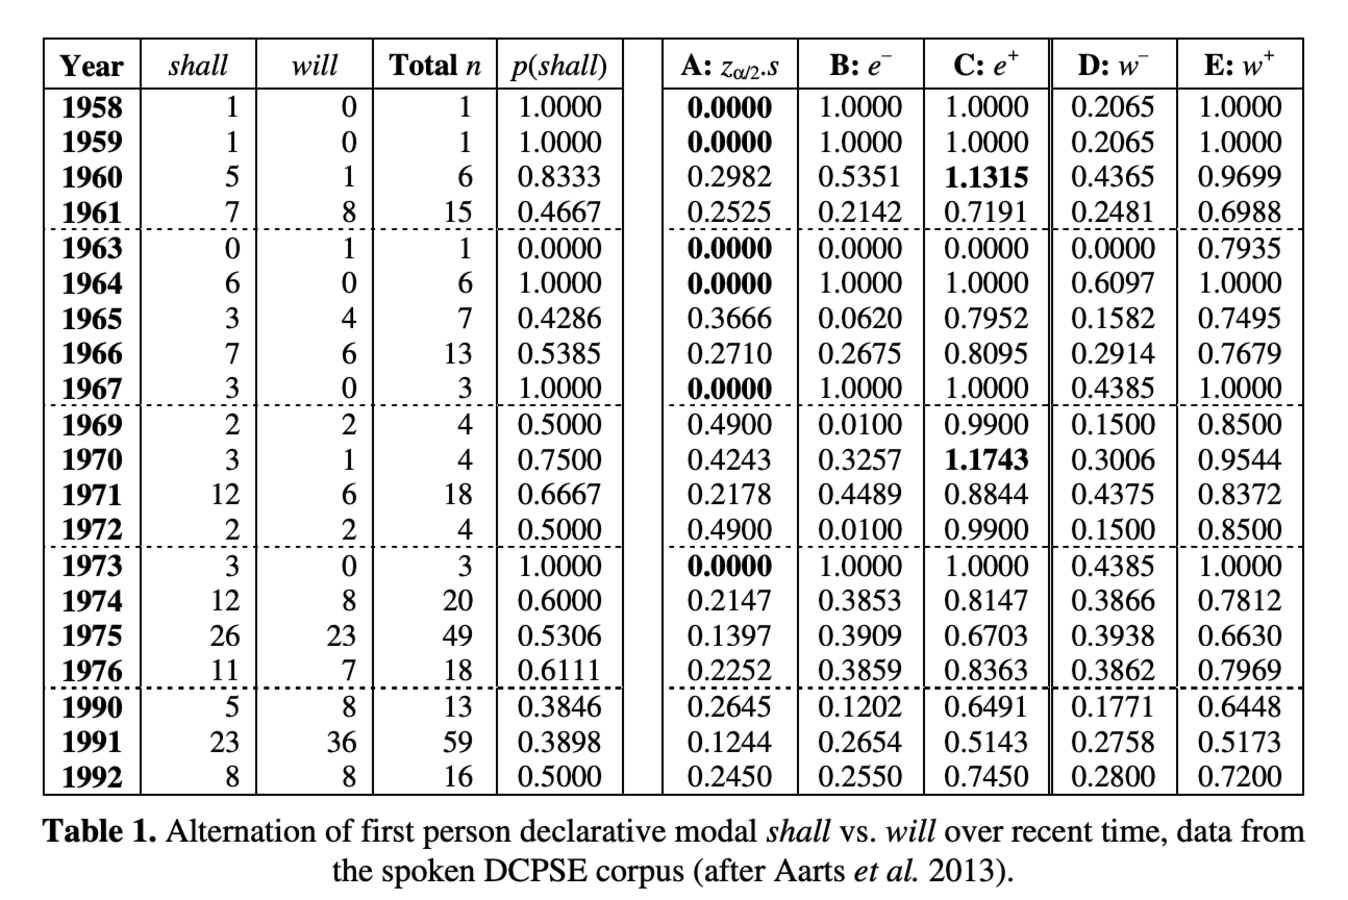
\includegraphics[scale=0.4]{wilson_chart.pdf}
    \caption{A paper about confidence intervals published a chart of values for
    the Wilson score interval~\citep{wallis2013binomial}, in the last two columns. Using $n$ and $p$
    for a $95\:\%$ confidence interval, we can quote this chart and compare with
    our code's output as a unit test.}
    \label{fig:wilson_chart}
\end{figure}

\subsection{Regression tests}
A regression test compares the result of a function against a previous
result from that function. The parallel implementation, in this case,
is the previous version of the same function.

There is a book called \emph{Release It!} that says we should
``make regression testing easy,''~\citep{nygard2018release}. It's hard to make it easy
because unit tests are built to test, not save output. Even if
they save output from functions, it takes work to figure out
\emph{how} a result changed if it did change. If the result
is a data frame, did every value change, or some subset?

While following the book's advice is a research project,
it's a good focus for any particular project to find places in the
code where regression tests would be most informative. Unit tests are
most absolute in their pronouncement when they test the simplest
functions. It's the mid-level functions, that do more work
and produce the more complex output, that benefit from regression.
The high-level functions will change output every time you touch
the code, but mid-level functions will change less frequently,
and there's a chance to guess why they changed.



\section{Testing parameter logic}\label{sec:parameter-logic}
\subsection{Introduction}\label{sec:parameter-introduction}
If we need to implement some matrix algorithm, then
we might make a function that has a few arguments: the matrix of data, algorithm parameters
to control cutoffs in the algorithm, and options to determine whether
the result is written back into the source matrix memory.
The data, algorithm parameters, and options are all, in the eyes of unit testing,
parameters.

These three kinds of parameters, however, tend to affect functions
differently. Options appear in the test of if--thens, so they change
the code path. The code path is the sequence of blocks of code that execute
for a particular set of parameters.
Algorithm parameters tend to appear in key equations, so that they
affect data flow in a function. The data flow is a graph
of which values in a function depend on which previous values.
The input matrix, itself, is effectively a two-dimensional matrix of
parameters, greatly increasing the number of possible inputs to a function.


\subsection{Decision Tables}\label{sec:parameter-decision}

Given that scientific functions have large spaces of possible inputs,
we have to choose which parameters and parameter
combinations to test, and we limit the tests by identifying
parameter values that are nearly-the-same test. For instance,
if a function calculates age-standardized mortality rate, then testing
the case where the mortality rate is 1.1 times larger hardly seems
a different test. Instead, we might ask how the function handles
missing values, zero values, or unusually sharp rises or falls in
mortality rate. Sets of parameters that probe the same faults in
the function under test are called \emph{equivalent.}

Methods to test parameter logic all have the same underpinning,
that they will try to test at least one set of parameters from
each of the equivalence classes of inputs. Deciding what is an
equivalence class can be difficult. Sometimes two parameters
sets are equivalent in terms of the mathematical statement of 
the model, but their representation in code makes one set
have a different risk from another. For instance, a function of small
values would be well-defined as an equation, but it could cause
denormalization when written in code.
It can also be the other way around, that
the mathematical statement of a model makes clear what parameter
sets may be equivalent. Information from both statements of
a function will be helpful.

A decision table is a list of parameters and the expected result
of the function, arranged with one unit test per row. The
tests can exhaust all possible parameter combinations or
can have a row per equivalence class, when the number of combinations
becomes large.

For instance, consider a function that projects a time series
using the trend of its running average. It could use the slope
of the last $m$ entries in the time series. It could weight
those last $m$ entries according to an exponential or Gaussian, so that
earlier entries count less. It could transform the entries
into log-space before projecting them. These options create
sets of allowed parameters.
\begin{center}
\begin{tabular}{|l|l|l|l|l|}\hline
$m$ & kernel & transform & range & output \\ \hline
5 & Gaussian & linear & 1.0 & 2.7 \\
5 & Gaussian & logarithmic & 2.0 & 1.9 \\
5 & exponential & linear & 3.0 & 2.8 \\
5 & exponential & logarithmic & 2.0 & 2.1 \\ \hline
\end{tabular}
\end{center}
The clear table is pleasing, but we can see that, even for
this small case, the list will be long. The example
above doesn't even begin to probe error conditions, such
as negative $m$ values or $m$ greater than the length
of the data. We might define equivalence classes for each
parameter, such as these.
\begin{center}
\begin{tabular}{|l|l|l|}\hline
parameter & \# cases & cases \\
$m$ & 5 & negative, 0, less than data, equal to data, more than data \\
kernel & 2 & Gaussian, exponential \\
range & 3 & negative, 0, positive \\
transform & 2 & linear, logarithmic \\ \hline
\end{tabular}
\end{center}
That makes $5 \times 2 \times 3\times 2 = 60$ cases.
The table also fails to mention the most important
parameter, the vector of data values.

If a parameter is a vector of numbers, what to test depends
even more on the particular math. Some suggestions:
\begin{enumerate}
    \item Set all values to a single edge case.
    \item Try monotonically-increasing or decreasing.
    \item Try non-increasing or non-decreasing (so that some
    consecutive values are the same).
    \item End points may be special, so test them separately.
    \item If the vector is, in some way, smooth, construct
    a vector where the maximum change, element to element, is no
    more than some prescribed value. See how large that value can
    be before the function fails.
    \item Orthogonal arrays are random draws of values that
    are spread out evenly through a multidimensional space.
    They are one way to explore the space of input arrays~\citep{Owen1992}.
\end{enumerate}
Each of these suggestions becomes another category for
equivalent inputs. If we used these five, then the total
number of tests above would be $60\times 6 = 360$.


\subsection{Limiting values of parameters}\label{sec:limits}

Not every parallel implementation is a brute-force retelling
of a model. Most mathematical functions provide finger-holds
support of their correctness.

The simplest of these are parameters for which a function
takes a known value. The function could be a mess of
polynomials of trigonometric quantities,
\begin{equation}
  y = (\sin x)^3 - 6 (\cos x)^2 + 2,
\end{equation}
but these simplify considerably at $x=0, \pi/4, \pi/2, \pi,$
and so on. If the function should divide by zero for some
number, then that, too, is a parameter for which the function
has a known value, an exception.

Another kind of limit is the distance between function results
as the function inputs get closer to each other. We can often
find faults in a function by testing continuity of the output.
Here, a good unit test would mirror the definition of Lipshitz continuity.
\begin{lstlisting}[language=python]
C = 2.0
for (x1, x2) in [(0, 1), (0, .1), (0, .001)]:
    assert f(x2) - f(x1) < C * (x2 - x1)
\end{lstlisting}
The \lstinline!C! variable is a bounds on the slope for any
pair of numbers.

Sometimes a limit of a function is the same limit you know
from high school precalculus,
\begin{equation}
  \lim_{x\rightarrow\infty} f(x).
\end{equation}
Maybe the limit goes to zero, or to 3, but the principle is
the same. You can test that a function is near the limit
as the value gets larger, or closer to zero. Better, you can
test that the function gets closer to the limit as the
parameter gets closer to its limit.

This is a game where incremental understanding of math
gives incrementally more careful attention to risk in the
function under test. We can know the limiting value of a
function, but we can also know how the function approaches
that limit. Another precalculus friend, the Taylor series
writes a function as a sum of terms that get smaller,
\begin{equation}
  f(x_0+x) \approx f(x_0) + \frac{f'(x_0)}{2}x + \frac{f''(x_0)}{6}x^2 + \epsilon.
\end{equation}
If we know the first term in the series, then the second term
is a good guess for how far the function's output should be from
the limiting value, as a function of $x$.


\subsection{Test Case Generation}
When we decide to use test-driven design, we start each bout of
coding by writing a test that mimics user input, and then we write
code until the application responds correctly to the user.
This is a high-level test, and it's an example of a test that
has many parameters because, for a scientific application, it
usually corresponds to adding a user-specified option to the
sum of the input data and configuration files. There is no
way to try every combination of inputs, and the application
may take a long time to run.

The luxury of combining every combination of input parameters
is called \emph{combinatorial interaction testing.} We usually
test some fraction of these possible inputs, called the
\emph{test coverage fraction,} not to be confused with the
term \emph{test coverage,} that refers to the percentage of
all code paths that are run at least once by any unit test.

How we choose which, of all possible tests, to run is a question
of test design, the same way a doctor designs a randomized
controlled trial or a botanist chooses treatments of plants
in a field. Let's look at how the most common choices
address risks in the code most efficiently.


\subsubsection{Random parameter choices}
Given a set of possible equivalence classes for each parameter, use a random
number generator to choose one of each. Do this as many times
as runtime allows. When using this method, it's critical to
report not only failing tests but also the exact set of parameters
that made the tests fail~\citep{arcuri2011random}.

Randomized test cases are easy to implement, and they can
supplant the author's duty to identify the greatest risks
in the code. The main drawback is time to run this kind of
test, especially because it's tempting to play the lottery
by letting it keep running.


\subsubsection{Combinatorial excursions}
If you decide that there is some most-common way to call
the function, set that as the baseline. Then loop over parameters,
trying all equivalence classes for each one. Then loop over pairs of parameters. Then sets of three. You define a limiting depth,
where the full combinatorial excursion is the case where the
limiting depth is the number of parameters.

These tests would be highly-biased towards that baseline parameter set.
It can make sense to define several most-important baseline
parameter sets from which to conduct combinatorial excursions.


\subsubsection{All pairs}
What if we could guarantee, that if we pick any two parameters
of a function, and we pick two values for those parameters,
that there is at least one unit test that includes that combination
of parameters? This is the all-pairs test design, to test
every possible pairwise interaction among parameters.
It packs these into as few tests as possible. For instance,
the same unit test might be the only time that pair
$(a=1, b=2)$ and pair $(c=3, d=4)$ appear, because their
pairwise interaction appeared in the same test.

All-pairs testing offers a feeling of completeness while
using many fewer tests than even a depth-2 combinatorial
excursion. There are claims that all-pairs testing almost
always finds every fault in a function that full combinatorial
excursions would fine~\citep{Pairwise}. It does not, however,
do any better a job than the randomized testing of emphasizing
particular parameter sets that the author decides carry
the most risk for a function or application.

The trick to using all-pairs testing is finding a library
that will compute the sets of parameters to use. Finding
those sets is, itself, an optimization problem.
While AllPairsPy works for Python~\citep{allpairspy},
and several papers cover algorithms~\citep{tung2000automating,pezze2008},
there are two articles that offer a friendly start~\citep{blass2002,czerwoka2006}.


\subsubsection{Stratification and filtering}\label{sec:parameters-stratification}
The sections above all imply that there could be some way
to emphasize which test are chosen, based on an assessment
of which parameters carry the most risk. For instance, if
a parameter is an option to make a copy of the input data
before further work, it would be enough to test that exactly
once, and not in all other parameter combinations. On
the other hand, there may
be certain parameter values that should be thoroughly-tested
because they challenge the numerical precision of the algorithm.

The ability to prefer tests of certain sets of parameter values
is called \emph{stratification.} That means you take any
of the test generation methods above and give the test author
the ability to weight which tests it should generate.

The throw out some of the generated tests is called
\emph{filtering.} Sometimes it's easier to generate tests
and toss useless ones than it is to generate the most-desired
tests in the first place.

Some of the more professional testing software includes
these capabilities, such as \textsc{aetg}~\citep{cohen1997aetg},
\textsc{cts}~\citep{hartman2004problems},
and the \textsc{act} library~\citep{kuhn2008automated}.


\subsubsection{All Other Methods}
The orthogonal arrays, mentioned in Sec.~\ref{sec:parameter-decision},
are yet another way to generate tests that span the space of
all possible parameters~\citep{Owen1992}.
Whichever method you choose, it's
good to have one of these methods available when it's time to
do user-level testing on scientific code.
\citet{petke2015practical} cover these strategies in their book,
and there are a few survey papers on the topic~\citep{nie2011survey,khalsa2014orchestrated}.


\subsection{Example}\label{sec:parameter-wilson}
This should use Wilson's Score Interval to guess standard error for a measurement~\citep{agresti1998approximate}.

This function finds standard error from effective sample size for two
different models. One is the binomial model, denoted ``proportion,''
and the other is a demographic rate, denoted ``rate,'' which is not bounded
by 1. For the binomial model, the Wilson score interval is
\begin{equation}
    \frac{\hat{p}+z^2/2n\pm z\sqrt{\frac{\hat{p}(1-\hat{p})+z^2/4n}{n}}}{1+z^2/n}
\end{equation}
where $z=z_{\alpha/2}$, so it's .975 for a $95\:\%$~confidence interval.
I think it will translate between confidence interval and standard
error by assuming asymptotic normality, which means assuming the
confidence interval is
\begin{equation}
    p\pm z \times\mbox{standard error}.
\end{equation}
This means a standard error from Wilson's score interval comes from
\begin{eqnarray}
    z \times\mbox{standard error} & = & \frac{z\sqrt{\frac{\hat{p}(1-\hat{p})+z^2/4n}{n}}}{1+z^2/n} \\
    \mbox{standard error} & = & \frac{\sqrt{\frac{\hat{p}(1-\hat{p})+z^2/4n}{n}}}{1+z^2/n}
\end{eqnarray}

For the standard error of a rate, there are two calculations, an asymptotic one
for large effective sample size and another for small effective sample size.
For large sample sizes, standard error is $\sqrt{\lambda/n}$, as expected for Poisson
rates. For small sample sizes, this code uses a linear interpolation between two values,
which are the large sample size value, pinned to $\lambda n=5$, and the value $1/n$.
\begin{equation}
    \left(1-\frac{\lambda n}{5}\right) \frac{1}{n} + \left(\frac{\lambda n}{5}\right)\sqrt{\frac{5/n}{n}}.
\end{equation}
A larger selection of standard estimators for Poisson rates is in \citet{patil2012}.

%https://stash.ihme.washington.edu/projects/CC/repos/cascade_ode/browse/cascade_ode/drill.py
\begin{lstlisting}[language=Python]
def se_from_ess(p, ess, param_type, cases=None,
                quantile=0.975):
    """ Calculates standard error from effective sample size
    and mean based on the Wilson Score Interval """

    err_msg = ("param_type must be either "
               "'proportion' or 'rate'")
    assert param_type in ['proportion', 'rate'], err_msg

    if cases is None:
        cases = p * ess

    if ess == 0:
        return 0

    if param_type == "proportion":
        z = stats.norm.ppf(quantile)
        se = np.sqrt(p * (1 - p) / ess + z**2 / (4 * ess**2))
    elif cases <= 5:
        # Use linear interpolation for rate parameters
        # with fewer than 5 cases
        se = ((5 - p * ess) / ess + p *
              ess * np.sqrt(5 / ess**2)) / 5
    elif cases > 5:
        # Use Poisson SE for rate parameters with more than
        # 5 cases
        se = np.sqrt(p / ess)
    else:
        raise Exception(
            "Can't calculate SE... check your cases parameter")

    return se
\end{lstlisting}

\begin{center}
    \begin{tabular}{ll}
    \hline
    Variable & Possible Values \\ \hline
    mean $p$ & $p<0$, $0<p<1$, $p=0$, $p>1$, single value or array \\
    effective sample size $e_{ss}$ & $e_{ss} <0$, $0<e_{ss}<p/5$, $e_{ss}>p/5$ \\
    param type & proportion, rate, other \\
    cases & missing, None, negative, $<5$, $5$, $>5$ \\
    quantile & missing, $0<q<1$, $q=1$, $q>1$ \\ \hline
    \end{tabular}
\end{center}
The decision table will be quite large, but we can start with some
particular values.
\begin{center}
    \begin{tabular}{llllll}
    \hline
    mean & ess & param type & cases & quantile & result \\ \hline
    0.04 & 100 & rate & missing & 30 & $0.02$ \\
    0.04 & 100 & None & missing & missing & assertion \\
    0.04 & 0 & rate & missing & missing & 0 \\
    (0.04, 0.01) & (0, 0) & rate & missing & missing & (0, 0)
\end{tabular}
\end{center}

This function is written to handle an array of mean values.
If the input mean is an array of numbers and the standard error
is zero, the output of the function is a single zero, not an array
of zeroes.

\subsection{Conclusion}
If you can separate parameter handling from the rest of the code,
you can test better. The idea is to transform from input parameters
that are user-friendly to those that are simpler for the algorithm
to use.
Think of parameter-handling as translation from an external
     language to some kind of parameterization that's more
     consistent, concise for internal processing.


\section{Mutation testing}\label{sec:random-changes}
The function under test, as with any block of code, can be
represented as a syntax tree. This tree of operators, operands,
and assignments, represents a contract with the compiler,
represents the flow of information from parameters to output,
represents a treasure map of potential faults. There is a form
of testing that reads the function under test, creates its
syntax tree, and randomly mutates it. At random, it adds a one to the
limit of a loop, and runs the unit tests again. It changes
the order of assigment statements and tests again. Each time
it records the change to the tree, and the outcome of the tests.

When the test suite is mature, then there should be some test
that fails for each mutation, but that isn't the case. A
large percent of genetic mutations of the code that
cause no test to fail, and most of those won't indicate the
code has a fault, or even that tests are incomplete. Instead,
these cases force a question about what choices in the code
matter and what is irrelevant.

We discussed in Sec.~\ref{sec:parameter-introduction} that
we can understand a function by parsing it as a code path
or as a data flow. Each random mutation to the code will
have an effect that traces backwards to the input parameters
or forwards to the result, through code paths and data flows.
When a mutation has no effect on tests and isn't a fault,
it highlights the conditionals that it affects later in the function
and the values it affects later in the function.

What we discover, when we look at those conditionals and
values, is that mutations won't be faults when they don't
break invariants in the code that are enforced by more than
one mechanism. For instance, they may set a value that is
later overwritten, not read. They may change the length
of an array, but later for-loops iterate only over a smaller
portion of the array.

It's normal for a function to accidentally doubly-enforce
the invariants it needs to be true. It's normal for this testing
technique to tell you, once for each of thousands of iterations,
that either your test coverage is incomplete or that
code will sometimes work fine after your cat walks across
the keyboard.


\section{Testing data movement}\label{sec:data-movement}

\subsection{Data movement}\label{sec:movement-movement}

We said in Sec.~\ref{sec:parallel-twice} that there are four
steps to writing a scientific function, representing the mathematical model,
preparing a discrete version, translating it to algorithms,
and writing the code.
Rarely is scientific software just one mathematical model
and just one ensuing algorithm. It's a series of models supported
by a series of algorithms.

For this software, as for any software, using the right algorithm
ensures speed and scalability, and the right algorithm depends on
its associated data structure. The relevant undergraduate class
is called Data Structures and Algorithms, always the two together.
As a result, performant scientific code is a series of algorithms
joined by a series of translations from one data structure to
another, each to support the next algorithm. The high-performance
computing crowd calls any such code \emph{data movement,} as though
it were replacing sets in the entracte,
but software engineers call it integration code and know that
integration testing is one of the most important kinds of unit test.


\subsection{Integration testing data movement}

A classic example of data movement is reorganizing a multidimensional
array from one axis ordering to another. An algorithm with nested
for-loops usually acts on nested axes. The order of the axes should
put those for the inner loops last (for \textsc{c} and Python which are row-first), or put those
same axes first (for \rlang and Julia which are column-first). This so
often controls the speed of an algorithm that it isn't considered an 
optimization to fix it but an error to fail to set the order.

More complicated an example would be translating a graph from
an edge-list representation to an adjacency matrix representation.
Both have their place, but the correct form depends on the
algorithm that will act on this data.

Data movement tends to stress performance of memory access
and integer arithmetic. It carries risks of off-by-one errors,
loop endpoint errors, and assignment errors. These are different
from the performance characteristics and likely faults in core
algorithmic code, so they suggest data movement should be in its
own function and should be tested separately, for both performance
and efficient testing.

This produces a mental model for a scientific application. It begins
with translating configuration parameters from their specification
to the values internally. Inputs are verified. Then the application
is a series of data movement, followed by algorithm, and data movement
for the next algorithm. Then results are written.

\subsection{The CRUD case}\label{sec:crud}

The prosaic brother to data movement is the ubiquitous selection
and editing of data frames when reading and writing data.
The data frame is the algorithmic equivalent of a minivan, more
about convenient pickup and drop-off than about getting from $A$
to $B$. When we edit data frames, during save or load, or during
data movement, the correct result is more a matter of software specification
than a matter of difficult calculation.

A good testing method for data frame manipulation, is therefore
unit tests that assert the output data frame meets a list of requirements.
There is, happily, a framework
for recording and conveying this work, the create-read-update-delete
(CRUD) list. For example, if we were editing a mortality data frame:
\begin{itemize}
\item \textbf{Create} - If the input data doesn't have excess mortality,
  then derive it from cause-specific mortality and prevalence.
\item \textbf{Read} - If the user specifies \lstinline!get_csmr!, then get cause-specific
  mortality from the database and add it to the data.
\item \textbf{Update} - Use the average of incidence data at all child
  locations because it tends to be sparse.
\item \textbf{Delete} - All-cause mortality isn't included in this step.
\end{itemize}
These are requirements. Failure to meet one of these requirements
often won't make the code stop running. It's no less wrong.

These tests are classic boundary-value tests, where
we try parameters at the lower boundary, upper boundary,
and middle of the range. Combinatorial testing can be appropriate
across all parameters, and we can often create a single data frame
where each row represents a different test.

\subsection{Example}
This example, in Python, is a function with two arguments, but both
are dataframes, just read from input files. Think of them as two spreadsheets
with multiple rows and column headers \lstinline!x_local!, \lstinline!a_data_id!,
and so on.
\begin{lstlisting}[language=Python]
def shift_priors(self, data, adj_data):
    """For subnationals, shift priors given parent run.

    Args:
          data (pd.DataFrame): All of the input data, including priors.
          adj_data (pd.DataFrame): Parent predicted data values.

    Returns:
        Data with adjusted priors.
    """
    integrands = data.integrand.unique()
    priors_from_draws = data[data.x_local == 0]
    unadjusted_data = data[data.x_local == 1]
    parent_predict = adj_data[
        (adj_data.x_local == 1) &
        (adj_data.a_data_id != IHME_COD_DB) &
        (adj_data.location_id == int(float(self.loc)))]
    shifted_priors = pd.DataFrame()
    for ig in integrands:
        ig_prior = priors_from_draws[priors_from_draws.integrand == ig]
        ig_data = parent_predict[parent_predict.integrand == ig]
        if len(ig_prior) == 0:
            pass  # No priors to adjust
        elif len(ig_data) == 0:
            # No fit with which to adjust, so keep the priors.
            shifted_priors = shifted_priors.append(ig_prior)
        else:
            ig_prior -= ig_data.mean()
            shifted_priors = shifted_priors.append(ig_prior)

    shifted_priors['meas_value'] = shifted_priors.meas_value.clip(lower=0)
    newdata = unadjusted_data.append(shifted_priors)
    return newdata
\end{lstlisting}

If we wanted to make a decision table for this function, what are
the possible values of each entry in each row of the input data?

\begin{center}
\begin{tabular}{|l|l|}
\hline Variable & Values \\ \hline
\lstinline!data.x_local! & 0, 1, not 0 or 1 \\
\lstinline!data.integrand! & same as another row, same as adjusted row \\
\lstinline!adj_data.x_local! & 0, 1, not 0 or 1 \\
\lstinline!adj_data.a_data_id! & \lstinline!IHME_COD_DB! or not \\
\lstinline!adj_data.location_id! & \lstinline!self.loc! or not \\
\lstinline!adj_data.integrand! & same as another row, same as data row \\ \hline
\end{tabular}
\end{center}

\noindent{}That makes $3\times 4 \times 3\times 2\times 2\times 4=576$ different inputs.
This excludes the effects of calling the function
\lstinline!adjust_prior_by_mean_of_fit()!.

What is the algorithmic complexity of this function? There is one
if--then--else, so the answer could be three, but each condition in a dataframe
selection is another path through the code. For instance,
\lstinline!data.x_local == 0! is a conditional with two outcomes, leading
to very high algorithmic complexity, hidden in data frame arguments.

A project manager can ensure good communication between the scientist and
developer by writing \textsc{crud} assertions in English.
\begin{itemize}
    \item[R1.] Read parent location's estimate of priors as ``adjusted data.''
    \item[U1.] Update adjusted data so that the mean of the priors for this location matches
        the mean of the data for this location. Keep the shape of the priors.
    \item[U2.] Update priors, after adjustment, so that they are greater
        than zero for all integrands.
    \item[D1.] Delete local adjusted data that doesn't match the current location.
    \item[D2.] Delete local adjusted data that doesn't match the integrands.
    \item[D3.] Delete local data for this location if there are no parent
        priors for the same integrand.
\end{itemize}
Then we can write tests that verify these \textsc{crud} requirements for
each of the 576 kinds of inputs.



\section{Using symmetry to test a function}\label{sec:symmetry-test}

Sometimes knowing the math of a software function lets you
test the software, even when you have an oracle problem.
\emph{Metamorphic testing} uses the symmetry of the math function
in order to test the correctness of the software function~\citep{ding2016,guderlei2007,kanewala2015,liu2014}.

The mathematical description of a function is that it relates
a domain (input) to a range (output). We write $f(x) = y$.
If the function is an exponential, then $e^{-x} = 1 / e^x$,
so $f(-x) = 1 / f(x)$. We may not know what the value of
$e^{2.4}$ is, but we do know it has to match $1 / e^{-2.4}$.

Here's a longer example. Given a mortality rate, $m$, the
mean age of death over an age interval, $n$, is
\begin{equation}
    a = \frac{n - n(1+m n)e^{-m n}}{1 - e^{-m n}}.
\end{equation}
If we notice that this equation can be written
\begin{equation}
    a = f(m, n) = n  f_1(m  n),
\end{equation}
then we can design an interesting test.
\begin{eqnarray}
    \frac{a}{n} &= &f_1(m  n) \\
    \frac{a/2}{n/2} &= & f_1((2  m)  (n / 2)) \\
    a /2 &= & (n/2) f_1((2  m)  (n / 2)) \\
    a &= &2 * f(2m, n/2) \\
    f(m, n) & =& 2 * f(2m, n/2)
\end{eqnarray}
This result isn't true for almost all functions. It's a strong test
of the implementation. It's an example of the more general
form of symmetry testing, which insists that some transformation
of the inputs has a relationship with some transformation of the 
outputs,
\begin{equation}
    f(g(x)) = h(f(x)),
\end{equation}
where $f$ is the function under test, and $g$ and $h$ are the transformations.

\begin{lstlisting}[language=R]
mean_age_of_death <- function(m, n) {
  (n - n * (1 + m * n) * exp(-m * n)) / (1 - exp(-m * n))
}
test_that("dividing by a constant multiplies by a constant", {
  m1 <- 0.01
  n1 <- 1.0
  a1 <- mean_age_of_death(m1, n1)
  for (k in seq(0.1, 5, 0.3)) {
    a2 <- mean_age_of_death(k * m1, n1 / k)
    expect_lt(abs(2 * a2 - a1), 1e-7)
  }
})
\end{lstlisting}

Metamorphic testing is an assertion about a symmetry relationship between
the domain and range of a function. Because it's an invariant at the top-level
of the function, it has an opportunity to find simple faults in algebra,
grouping of terms, or off-by-one errors. It also has an opportunity to
find faults that result from denormalization or loss of significant digits
in floating-point math.


\begin{callout}
\textbf{Mathematical Complexity}---Has your code editor ever told you,
"Computational complexity 16, project limit is 15. Please refactor?"
\emph{Computational complexity} looks at every if--then--else and counts the
number of possible paths through a function.
Scientific code has high \emph{mathematical complexity,\/} which is a
count of the number of mathematical operators and function calls in
a function. Would you want your linter to insist on low mathematical complexity in
a function?
\end{callout}


\section{Testing the compiler}\label{sec:test-compiler}

Let's say you have a cluster of computers. They are all Intel machines,
but they come from different years. They could be different architectures
or just different steppings of the \cpu, which is the least difference
one can have between two chipsets. You compile code on one machine,
or you install some \rlang package that compiles code underneath. When
you move to another computer on another day, that same code fails
to run with the message, ``invalid opcode.''

An opcode is a machine-language instruction. The computer you used
yesterday knew a command that's slightly too fancy for the computer
you're using today, and it failed. You have to clean out the code
and recompile today. It's not that the new computer is just older.
It's still possible that, were you to switch back, there might be
the same message again. The history of \cpu opcodes isn't a forward
march into a larger, better set.

That scenario would be annoying, and it's a headache for people
saddled with heterogenous clusters. They solve it with, for instance,
creating architecture-specific shared drives so that they can
install a different version of the software for each version of
system architecture on the cluster. That scenario is, however, a
best case scenario.

The worse scenario, and I wish this were rarer, is that the
software runs on the other computer but gives the wrong error.
It can fail silently. This seems like an abrogation of a compiler's
contract with its faithful coder, but it isn't. That compiler
ensured that the code ran well enough on one target architecture.
The problem is that compiler optimizations at level \textsc{o3}, and above,
are willing to make slightly riskier choices that yield great
performance benefits. These choices are tuned to the architecture
at hand, or as requested by compiler options, and, while they may
run on similar architectures, carry more risk of error on them.
It solves the problem of having languages
that don't clearly represent time-saving invariants and of coders
who can't afford motorcycles.

There's a solution for this, too. Turn all optimizations down
to \textsc{o2} or lower. Or claim to the compiler that the \cpu
understands no later than the \textsc{sse2} instruction set from 2000.
Unless you're intentionally commemorating the year Phil Katz died, you'll see
this as a severe loss of performance.

The last option to deal with this problem is called acceptance
testing. It means that you create a test to run before you
run code on a new machine. It won't do the work of creating
a separate version of the code, if needed, but it tells you if
you need it. You don't generally care about integer performance
here. You care about vectorized code and floating-point code.
That's where the problems will be, so you can subset the test
suite for these acceptance tests.

Designating a subset of all tests as acceptance tests is an
example of test case prioritization~\cite{rothermel1999test}.
We prioritize tests by hand, by marking tests to be run under
different conditions, but tests for scientific code can be lengthy,
which makes it worth considering automatically reordering tests
so that those that are most sensitive to correctness run by 
themselves, or run first~\cite{yoo2012regression}.


\section{Outside the code}\label{sec:outside-code}

\subsection{Documentation defines what a function wants to be}

Sec.~\ref{sec:parameter-wilson}, on parameter testing, uses a function that's a hybrid
between Wilson's score interval and a Poisson estimator. That hybrid
doesn't have a name, and there's no paper or Wikipedia entry for it.
We can test that its output is a continuous function of its input
parameters. We can test that it matches known values for limiting cases,
but the right version of this function is the one that a team agrees
is right.

That team is usually not just the people in the room. It includes stakeholders
outside the room. It includes reviewers. It includes future versions of the team.

The tests can be a clear statement of the contract this function upholds.
So, too, can project documents, as mentioned in the data movement section,
where \textsc{crud} defines selection from a dataframe. 
Function documentation, in particular, is where the software
developer, the one who wrote the function, states their understanding
of the contract that function fulfills. It's the closest statement,
in English, of what unit tests should assert.

Like all other work, documentation takes time and is prioritized by
how it addresses risk. Give the highest-level explanation first.
This could be a reference to a paper, a book section, documentation from another library.
Then say \emph{why} this function exists and \emph{why} it works the
way it does.

And on the technological side, equations in documentation communicate
clearly with research-oriented readers. Similarly, code examples, run
as unit tests themselves, within the documentation, ensure always-working
examples for development.


\subsection{Team is critical to tests}

Take a function under test and project it onto a
screen at the front of a meeting room. Place around that screen
the team you have or the team you would like to have.
Engineering studies show that the future utility, or burden,
of that function depends no more on its testing than it
depends on the culture of that team~\citep{neumann2016,kanewala2014}.

Culture is beyond the scope of this document, but conversations
aren't. One point to raise in that meeting room could
be the effect of discretization or floating point representation
on the mathematical representation. Another could be a
description of statistical properties of the function, a set
of equations, beyond those to implement the function, that
describe its expected behavior. Someone could raise an observation
that brute force solution is suprisingly possible.
The team could discuss likely sets of parameters that might
matter, some determined by the math, some by logic in the
code. A product manager could supply \textsc{crud} requirements.
A systems engineer could describe the expected architectures
and risk of failure due to optimization levels. Every section
of this document is a prompt for conversation.

Testing well is helpful, but we saw, in the section about
data movement, that identifying what is data movement
and what is an algorithm meant we could label the two.
Giving a function a good name is important to a software
developer, but scientific code is rarely owned by a team
of software developers. It's shared by a team of researchers.
That team has a body of knowledge about the software, and,
the same as any body of knowledge, it's a shared set of
understanding where new things are added and less useful
ideas are dropped.

In this research environment, collaboration on testing
creates commonly-understood, trusted functions. This shared
agreement on the (tested) entities with which we do our work, more
than any single snapshot of the whole calculation, are
what the group understands about the code. These trusted
functions will be copied into other projects, translated
to other languages. They will exist long beyond the work
that has your name.

\section{Further Reading}\label{sec:further-reading}

The most complete books on general software testing offer a sound
basis for testing any kind of code. I recommend starting with
\emph{Software Testing: A Craftsman's Approach,}~\citep{jorgensen2013},
while skipping its chapter on set theory, and then taking a look at
\emph{Software Testing and Analysis: Process, Principles, and Techniques,}~\citep{pezze2008},
if you haven't had enough.

The complexity of scientific code not only makes it difficult
to test but also mummifies past working code. Lest such a mummy
come to life in your hands, look at \emph{Working Effectively with Legacy Code,}~\citep{feathers2004working}.

There are several sources directed at scientific developers, for
construction of code, as well as testing. These are some recent highlights:
\begin{itemize}
	\item \emph{Software Engineering for Science,}~\cite{carver2017}.
	\item ``Testing Scientific Software: A Systematic Literature Review,''~\cite{kanewala2014}.
	\item ``Development of Scientific Software and Practices for Software Development: A Systematic Literature Review,''~\cite{neumann2016}.
\end{itemize}

\appendix

\section{Faults in Mathematical Code}\label{sec:faults-and-failures}

For each section, ask what faults does this technique limit?
For instance, using a limit test for constant-mortality mean age
ensures you don't have a numerical fault.

\subsection{Fault versus Failure}
Jorgensen's \emph{Software Testing: A Craftsman's Approach} distinguishes
faults from failures~\citep{jorgensen2013}.
A fault is the characters that were typed
incorrectly. A failure is observation that something went wrong.
For instance, there may be a fault that 0.3 is assigned to an integer
instead of assigning it to a double. The failure will happen later,
in the code that divides $1 / 0$.

Any failure is a problem. We don't want to throw exceptions or segfault.
Worse for mathematical code is when an error in the code isn't visible
but does give a wrong answer.
The worst problem is faults that aren't failures.


\subsection{Classes of Faults}
Jorgensen gives a set of fault categories and examples, elided here:
\begin{itemize}
    \item Input/Output - incorrect input accepted, incomplete result
    \item Logic - missing cases, test of wrong variable
    \item Computation - incorrect algorithm, parenthesis error
    \item Interface - parameter mismatch, call to wrong procedure
    \item Data - Incorrect type, wrong data, off by one
\end{itemize}
These all apply and, yes, read Jorgensen, but most of this article 
expands upon a single category of fault: incorrect algorithm.

This document covers two different kinds of failure-free faults.
\begin{itemize}
\item Simple data manipulation that doesn't do what the user
   expected it to do.
   
\item Mathematical functions that return a result that looks
   reasonable but isn't correct.
\end{itemize}
While these faults are within the taxonomy of faults
in any book on testing, we can discuss some of the particular
challenges that complicated mathematical functions introduce.

\bibliography{tsci}
\end{document}
